\documentclass[12pt]{article}
\usepackage{amsmath, amsfonts, amssymb, amstext, amscd, amsthm, graphicx, mathtools,mathrsfs}
% I use these packages so frequently that I include them in nearly all my files
\usepackage[framed,numbered]{matlab-prettifier}
\usepackage[T1]{fontenc}
\usepackage[notextcomp]{kpfonts}
\usepackage[pdftex,hidelinks]{hyperref} % To create hyperlinks in text
\usepackage[margin=0.5in]{geometry} % Creates better margins and lines for documents
\usepackage{tikz}
\usepackage{cite}
\newcommand{\R}{\mathbb{R}}
\newcommand{\eps}{\varepsilon}
\newcommand{\outerprod}{\operatornamewithlimits{\bigcirc}}
\title{Multilinear Alternative to Proper Orthogonal Decomposition: Notes on the HOSVD}
\author{Daniel Sharp}
\date{\today}
\begin{document}
    \maketitle
    \section{Introduction}
    In partial differential equations (PDEs), analytically solvable problems are far and few between in higher dimensions, giving ample reason for development of numerical solutions. However, even numerically approximating a solutions in several dimensions is significant work: many software packages geared toward solving these complicated PDEs are sold to engineering firms for this express purpose, frequently intended for powerful computers or compute clusters. Additionally, once a solution is developed for a given set of variables, it is ostensibly only useful for that solution. Reduced Order Models (ROMs) are developed for this express phenomenon. One method of developing a ROM is to ``linearize'' the problem in a sense, developing a basis of functions in some parameter or group of parameters and then looking linear combinations of that basis of functions. A popular method of solution is the ``Proper Orthogonal Decomposition.'' This decomposes a series of snapshots of a PDE's solution into orthogonal discrete parts, which form a basis for the spatial component of the PDE solution. This frequently uses the method of taking the Singular Value Decomposition (SVD), or some variant, to find the ``best'' basis.

    A very robust technique, taking the SVD of large matrices and compressing the data through truncation is near-optimal numerically in many situations. However, it's only defined on a two dimensional space-- complicated PDEs depend on many more variables and parameters. In addition to space and time parameters, there are frequently other parameters perturbing the system in the initial or boundary conditions. we examine the HOSVD, a Tucker-style extension of the SVD for tensors, to exploit and explore this dimensionality. All numerical experiments were performed in MATLAB, frequently using abilities within TensorToolbox provided in \cite{ttb}. All substantial code used for creating this paper is found on GitHub \underline{\href{https://github.com/dannys4/hosvd_pde_exploration}{here}}.

    \section{Theory}
    For an extensive discussion of how the POD relates to the SVD, see \cite{pod_book}. However, a brief description is provided here. The POD is used in reducing data about the solution of a PDE into a meaningful structure, frequently using a truncated SVD (see \cite{trefethen_bau} for details). Additionally, the SVD is known to create effective bases for the domain and range of a finite dimensional linear operator, which is this ``meaningful structure'' mentioned above, where the vectors are ordered such that they optimize the variation in each dimension. However, the problem with the SVD is that it can only work on finite dimensional linear operators. Fredholm theory and integral transforms, at the very least, creates an ostensible extension to this for compact linear operators \cite{kreyszig}, and using the SVD to approximate any functional basis using finite element methods or finite difference methods would get a decent approximation of the compact linear operator.

    A discussion of tensors is now necessary to introduce the vocabulary and strategy of the general topics. First, a tensor $\mathscr{T}$ is called \textit{order}-$d$ or \textit{mode}-$d$ if there exist $n_1,\cdots,n_d$ such that $\mathscr{T}\in \R^{n_1\times\cdots\times n_d}$. Here we use the term ``mode'' to avoid any confusion with the connotation of ``order'' with regards to analysis and differential equation techniques. The $(j_1,\cdots,j_n)$ entry of $\mathscr{T}$ is denoted $t_{(j_1,\cdots,j_n)}$. Then define the $i_k$th \textit{slice} in mode $k$ to be $\mathbf{T}_{i_k,k}\in\R^{n_1\times\cdots\times n_{k-1}\times n_{k+1}\times\cdots\times n_d}$ which includes all entries $t_{(j_1,\cdots,j_{k-1},i_k,j_{k+1},j_n)}$ ordered as in $\mathscr{T}$ (note that $i_k$ is fixed). We define tensor-vector products much like \cite{kolda_bader} where we see
        \[\mathscr{T}\times_k \mathbf{v}^T = \sum_{i_k=1}^{n_k}v_{i_k}\mathbf{T}_{i_k,k},\]
    where $\mathbf{v}\in\mathbb{R}^{n_k}$. Now, suppose $\mathbf{A}\in\R^{m\times n_k}$ where $\mathbf{A}$ has $j$th row $\mathbf{a}_j^T$. We define $\mathcal{P} := \mathscr{T}\times_k\mathbf{A}$ such that $\mathbf{P}_{j,k} = \mathscr{T}\times_k \mathbf{a}_j^T$. Finally, we denote the \textit{outer product} of a tensor and a vector as $\circ$. Let $\mathbf{v}\in\R^{n_{d+1}}$, and $\mathscr{P} := \mathscr{T}\circ\mathbf{v}$. We define $\mathscr{P}$ to satisfy $\mathscr{P}\in\R^{n_1\times\cdots\times n_d\times n_{d+1}}$ and $\mathbf{P}_{j,d+1} = v_j\mathscr{T}$ (these definitions are equivalent to those of \cite{hosvd, kolda_bader}). We now have the tools to build the formal definition of the HOSVD, given by the decomposition
    \begin{equation}\label{eqn:def_hosvd}
        \mathscr{T} = \mathscr{C}\times_1\mathbf{U}_1\times_2\cdots\times_d\mathbf{U}_d = \sum_{j_1=1}^{n_1}\cdots\sum_{j_d=1}^{n_d}c_{(j_1,\cdots,j_d)}\outerprod_{k=1}^d \mathbf{u}_{j_k},
    \end{equation}
    where $\mathbf{U}_k\in\R^{n_k\times n_k}$ (with \textit{columns} $\mathbf{u}_{j_k}$), is a matrix of orthonormal columns and $\mathscr{C}\in\R^{n_1\times\cdots\times n_d}$ has ``all-orthogonal'' properties described in \cite{hosvd}. We can lower the number of columns from $\mathbf{U}_k$ to some $m_k<n_k$ almost guaranteeing a sacrifice of true equality in favor of compression (depending on the properties of $\mathscr{T}$), and we call that the $(m_1,\cdots,m_d)$ multilinear-rank approximation of $\mathscr{T}$. In the case we use this multilinear rank approximation, we can make significant storage and complexity savings in calculation-- for example, if $m_k = n_k/4$, the ``truncated'' HOSVD would take up storage of order
        \[\mathcal{O}(\mathscr{C}\times_1\mathbf{U}_1\times_2\cdots\times_d\mathbf{U}_d)=\left(\prod_{k=1}^d m_k\right)+ \sum_{k=1}^dn_km_k = \frac{1}{4^d}\prod_{k=1}^d n_k+\frac{1}{4}\sum_{k=1}^d n_k^2 = \frac{1}{4^d}\mathcal{O}(\mathscr{T})+\frac{1}{2}\sum_{k=1}^d n_k^2,\]
    which can present significant savings for small $n_k$ and large $d$. If $m_k$ is even smaller in comparison to $n_k$ (as it frequently is in practice), we see much greater savings with less dependence on $d$.

    We propose the ``analytical'' HOSVD similar to a generalized Fourier series or truncated dyadic form of the SVD as an extension of this outer product above. Suppose we're given a real-valued function $f$ on some $d$-cell $I_d = [a_1,b_1]\times\cdots\times[a_d,b_d]$. Then, a multi-rank $(m_1,\cdots,m_d)$ analytical HOSVD of this is formally defined as
    \begin{equation}\label{eqn:hosvd_form}
        f(x_1,\cdots,x_d)\sim \sum_{j_1=1}^{m_1}\cdots\sum_{j_d=1}^{m_d}c_{(j_1,\cdots,j_d)}\prod_{k=1}^d \varphi_{j_k}(x_k),
    \end{equation}
    for some set of functions $\varphi_{j_k}$, where this relationship is equal if $f$ acts as a tensor on $\mathbf{x}$. In this case, it takes the form described in Equation \ref{eqn:def_hosvd}. Just as the discrete tensor case, we require $\langle\varphi_{j_k},\varphi_{j^\prime_k}\rangle_{L_2(a_k,b_k)} = \delta_{j_k,j^\prime_k}$ (the Kroenecker delta). We can represent the ordered set $\{c_{(j_1,\cdots,j_d)}\}$ as a tensor $\mathscr{C}\in\R^{m_1\times\cdots\times m_d}$.

    One problem would be the choice of what spaces $\varphi_{j_k}$ come from. The most natural thought from Fourier series would be to suggest that there exist a set of finite-dimensional function spaces $\{\mathcal{F}_k\}$, each of dimension $m_k$, such that  $\varphi_{j_k}\in\mathcal{F}_k$ for all $j_k=1,\cdots,n_k$. Then, $\{\varphi_{j_k}\}_{j_k=1}^{m_k}$ would form an orthonormal basis for this space of functions. Some examples of these spaces would be the span of the sets $\{\cos(j_kx)\}$, $\{x^{j_k}\}$, or $\{J_{j_k}(t)\}$ (where $J_{j_k}$ is a Bessel function of the first kind). The method to choose $\mathcal{F}_k$ is not discussed here; instead, the behavior is observed and different possibilities of $\mathcal{F}_k$ are heuristically discussed. This paper looks at the benefits of focusing on such an analytical method or a hybrid of the two methods.

    \section{Methodology and Performance}
    \subsection{Heat Equation}
    First, we start with a proof-of-concept relating to separable PDEs, such as the heat equation. Suppose we're given the PDE
        \begin{equation}\label{eqn:pde}
            \frac{\partial u}{\partial t}(t,x;p) = f(p)\frac{\partial^2 u}{\partial x^2}(t,x;p),\qquad u(0,x;p) = u_0(x,p),\qquad u_x(t,0;p) = u_x(t,1;p) = 0,
        \end{equation}
    which is a parameterized heat equation with Neumann boundary conditions. For a very simple case, suppose $f(p) = 1$ and $u_0(x,p) = p\cos(\pi x)$. Let $\theta(t,x,p) = pe^{-\pi^2 t}\cos(\pi x)$. Then,
        \[\theta_t(t,x,p) = -\pi^2pe^{-\pi^2t}\cos(\pi x) =\theta_{xx}(t,x,p),\]
    and we further see $\theta(0,x;p) = p\cos(\pi x) = u_0(x,p)$ as well as $\theta_x(t,x;p) = \pi pe^{-\pi^2 t}\sin(\pi x)$, so we know that $\theta(t,x;p)$ must satisfy the conditions to being a solution to this partial differential equation. The function $\theta$ acts like a three dimensional continuous analog of an outer product familiar to linear algebraists. Thus, intuitively, this result should form a 3 dimensional tensor that has some ``rank one'' property carrying over from the linear algebra intuition (and further discussed in \cite{hosvd,kolda_bader}). We then find the HOSVD of the solution analytically. Using the form described in equation \ref{eqn:hosvd_form},
        \[\theta(t,x,p)\sim\sum_{j_x=1}^{n_x}\sum_{j_t=1}^{n_t}\sum_{j_p=1}^{n_p}c_{j_x,j_t,j_p}X_{j_x}(x)T_{j_t}(t)P_{j_p}(p).\]
    However, by simple examination, we see this equality is exact with $n_x=n_t=n_p=1$, where $c$ is just the normalization factor for our solution's $X,T$ and $P$. Thus,
    \begin{equation}\label{eqn:heat_hosvd}
        \theta(t,x,p) = c X(x)T(t)P(p),\; \|X\|_{L_2(0,1)} = 1,\; \| T\|_{L_2(0,\tau)} = 1,\;\|P\|_{L_2(0,\psi)} = 1,
    \end{equation}
    where (down to a sign difference)
        \[c = \left\|\cos(\pi x)\right\|_2\left\|e^{-\pi^2 t}\right\|_2\|p\|_2,\;X(x) = \frac{\cos(\pi x)}{\left\|\cos(\pi x)\right\|_2},\;T(t) = \frac{e^{-\pi^2 t}}{\left\|e^{-\pi^2 t}\right\|_2},\;P(p) = \frac{p}{\|p\|_2},\]
    and $\|\cdot\|_2$ is the vector 2-norm over evaluation points (or $L_2$ norm if evaluated over an entire interval).

    Using finite difference approximation code based on \cite{pod_book,fin_diff}, we approximate the solution to (\ref{eqn:pde}) with $\Hat{\theta}(t,x,p)$. Then, we use the HOSVD function in \cite{ttb} to investigate the structure of $\Hat{\theta}(t,x,p)$. The result, with a tolerance of order $10^{-14}$ of relative error from the original tensor, has $\mathscr{C}\in\R^{1\times 1\times 1}$ (i.e. a constant), so all matrices decomposing this solution are then vectors. Now we look at what the analytical HOSVD of the solution is and compare the two. Numerically, we see that the core multiplier will have an error from our prediction of $1\%$. Then, in Figure \ref{fig:comp_heat}, we see the comparison between our prediction and the analytical results for each decomposition vector. Therefore, we conclude in this completely separable case that the HOSVD will approximate exactly what we expect the solution to be.
    \begin{figure}[t]
        \centering
        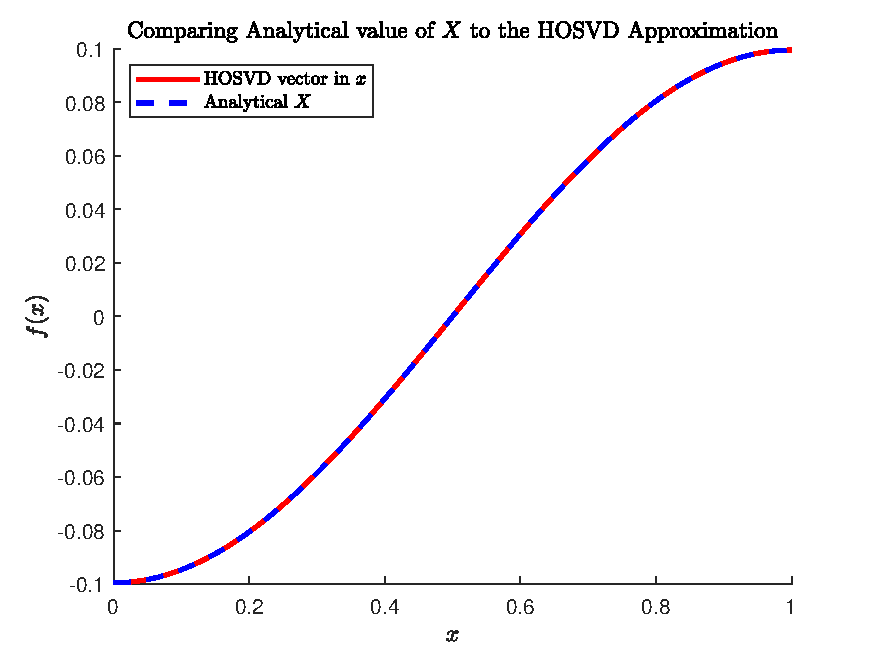
\includegraphics[width=0.49\textwidth]{figures/heat_eqn_comp_x.pdf}
        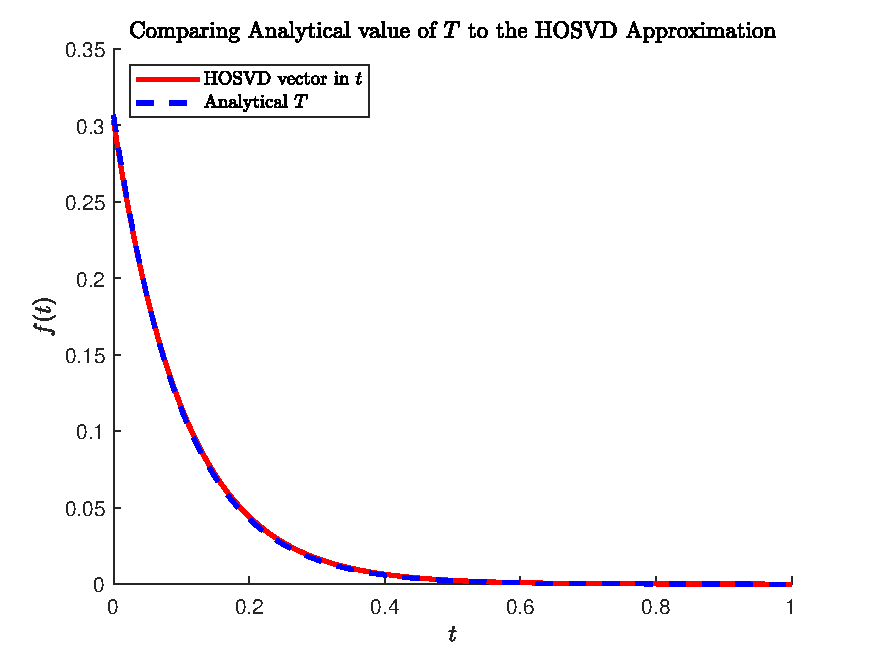
\includegraphics[width=0.49\textwidth]{figures/heat_eqn_comp_t.pdf}
        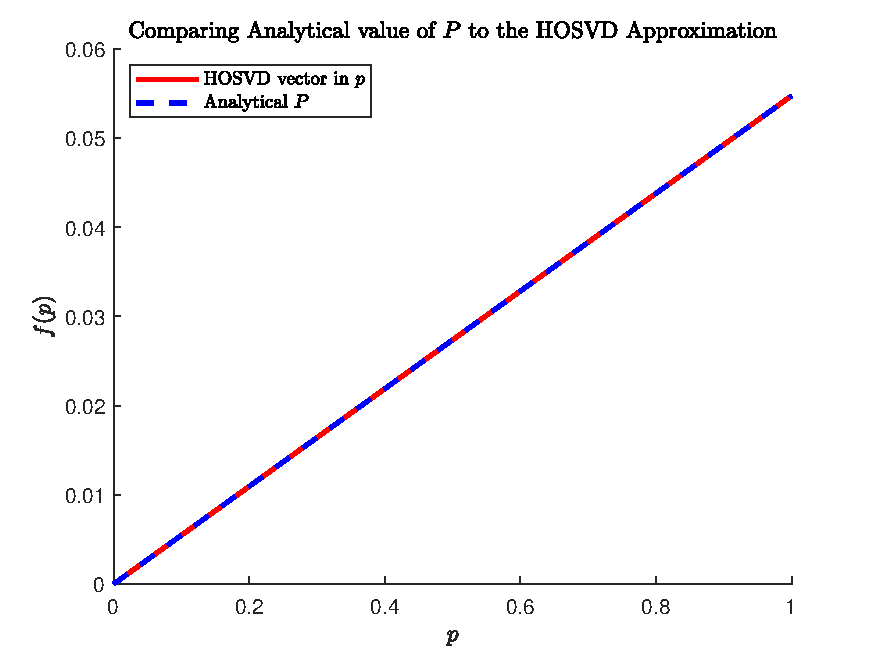
\includegraphics[width=0.49\textwidth]{figures/heat_eqn_comp_p.pdf}
        \caption{Comparing the elements of the HOSVD to analytical solution}
        \label{fig:comp_heat}
    \end{figure}

    We hypothesize the HOSVD is a method of approximating ``Separation of Variables'' for a numerical solution of a PDE (see a standard text on PDEs, such as \cite{pdes}, for information on Separation of Variables). This creates incredible potential for both compression and analysis of PDE solutions. For example, it is far less expensive to transmit a function $\theta(t,x,p)$ than it is to transmit the large tensor $\Hat{\theta}$. Additionally, since $\theta$ is continuous instead of the discrete $\Hat{\theta}$, we can extract more value from it. More generally, given a mode-$d$ solution $\mathscr{T}\in\R^{n_1\times\cdots\times n_d}$, we can approximate the HOSVD of $\mathscr{T}$ by approximating the singular vectors of $\mathscr{T}$ with $\varphi_{j_k}$ as seen in the notation of Equation \ref{eqn:hosvd_form}.

    \subsection{Burger's Equation}
    
    More rigorous tests of the above hypotheses and conjectures were conducted on a Burger-style PDE to understand some of the structure in a much less solvable environment. Examine the following PDE:
    \begin{align}\label{eqn:burger_def}
        \frac{\partial w}{\partial t}(t,x;\eps,q_1,q_2) = -w(t,x;\eps,q_1,q_2)\frac{\partial w}{\partial x}(t,x;\eps,q_1,q_2) + \eps \frac{\partial^2 w}{\partial x^2}(t,x;\eps,q_1,q_2),\\
        w(x,0;\eps,q_1,q_2) = \begin{cases} q_1\sin(2\pi x)+q_2\sin(4\pi x),&0\leq x\leq 0.5\\0, & 0.5\leq x\leq 1\end{cases} \nonumber\\
        w(0,t;\eps,q_1,q_2)=w(1,t;\eps,q_1,q_2) \nonumber,
    \end{align}
    which is not provided with any analytical solution. This problem's solution was simulated using a finite element codebase. The solutions were simulated for $q_1,q_2,x\in[0,1]$, $t\in[0,10]$, and $\eps\in[0.01,1]$, with equidistant chosen points and resolutions $n_x = 161$, $n_t=201$, $n_\eps = 20$, $n_{q_1} = 10$, and $n_{q_2}=10$. These simulations took several hours running on a 2017 HP Spectre x360 13 using an Intel i7-7500U CPU with 16.0 gigabytes of RAM for reference. The final solution tensor occupies about $494$ megabytes. However, the HOSVD with less than $0.07\%$ error of this solution tensor occupies only $2$ megabytes as it is of multilinear rank $(m_x,m_t,m_\eps,m_{q_1},m_{q_2}) = (28,35,7,10,4)$--- instead of choosing numerical values of $k=1,2,3,4,5$, we use the associated variables for clarity.

    \subsubsection{Structural Analysis of the Solution}\label{sec:structure}

    We first plot several of the $x$ singular vectors to examine the structure of $\Hat{w}\approx w$, our approximate solution, in $x$. Just examining the dimensionality, it seems that we can reduce the dimension in $x$ significantly compared to our original resolution.
    \begin{figure}[t]
        \centering
        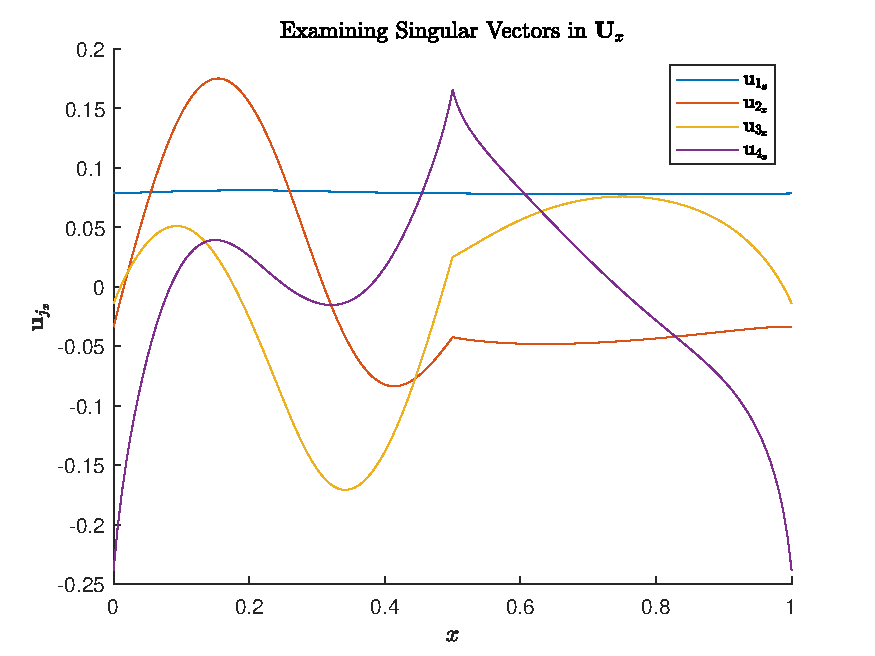
\includegraphics[width=0.48\textwidth]{figures/burgers_ux_1_4.pdf}
        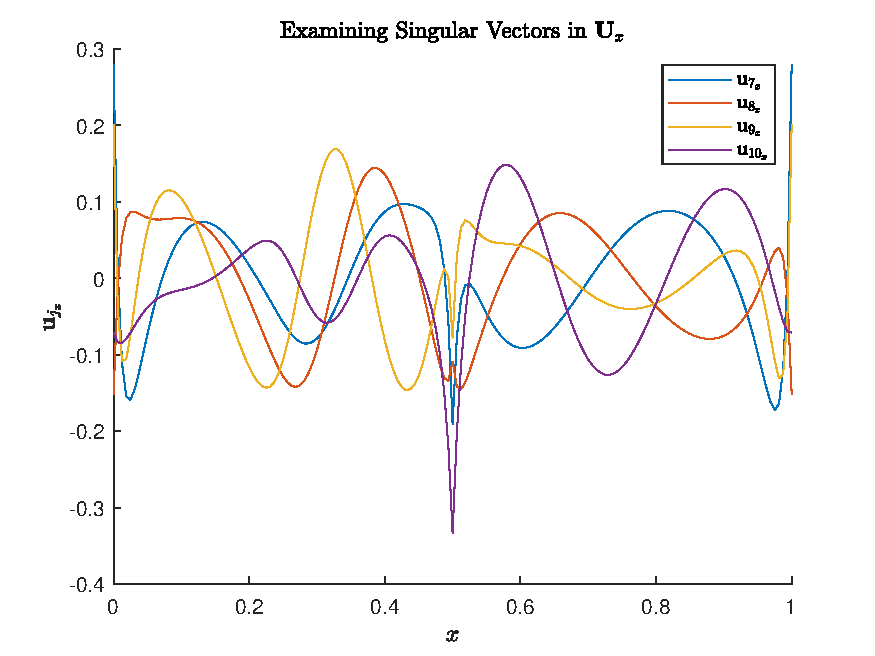
\includegraphics[width=0.48\textwidth]{figures/burgers_ux_7_10.pdf}
        \caption{Examination of $\mathbf{u}_{j_x}$ vectors}
        \label{fig:burgers_ux}
    \end{figure}
    In Figure \ref{fig:burgers_ux}, two groups of four columns from $\mathbf{U}_x$ are plotted and enumerated appropriately. Remarkably, these vectors have incredibly well-defined behavior, suggesting they are piecewise smooth functions. It's apparent from analyzing all columns, displayed and otherwise, in $\mathbf{U}_x$ that the matrix structure preserves the cusp-like quality at $x=0.5$ from the initial condition. In a solution, we would hope and expect for behavior that reflects such a significant quality in the given problem. However, there are no clear qualitative similarities for what space to use as $\mathcal{F}_x$ besides the obvious choice of spline functions. For the space of splines, we would have to establish appropriate points to use as knots for the support of the solution, since not every $\mathbf{u}_{j_x}$ has the same level or location of highest variation. Additionally, we see that many of the vectors are unbounded at the ends, which is problematic for creating a function with compact support.

    Similar to the columns of $\mathbf{U}_x$, the columns of $\mathbf{U}_t$ are somewhat well-defined but not easily identifiable as members of any conventional approximation space in Figure \ref{fig:burgers_ut}, most closely resembling a combination of Bessel Functions of both the first and second kinds or functions of the form like $\lambda e^{-\nu t}\sin(\tau t)$. We mention these functions as some of the vectors seem very large or unbounded near $t=0$. However, as a class of functions, we make some interesting notes. Relatively speaking, these solutions are much better at compressing in time than space, where $m_t<0.18 n_t$. We note additionally that all but the constant column of $\mathbf{U}_t$ asymptotically approaches zero. Third, all of the nontrivial columns oscillate at each value of $\Hat{t}$ between two different functions that are of similar shapes. The oscillation seems to be larger for less significant singular vectors, suggesting there might not be well-defined functions to approximate each of the vectors, preventing any analytical HOSVD. Overall, though, the vectors seem to at least have rigorous structure. Functions representing the structure could possibly bound the vectors presented in \ref{fig:burgers_ut}.
    \begin{figure}[t]
        \centering
        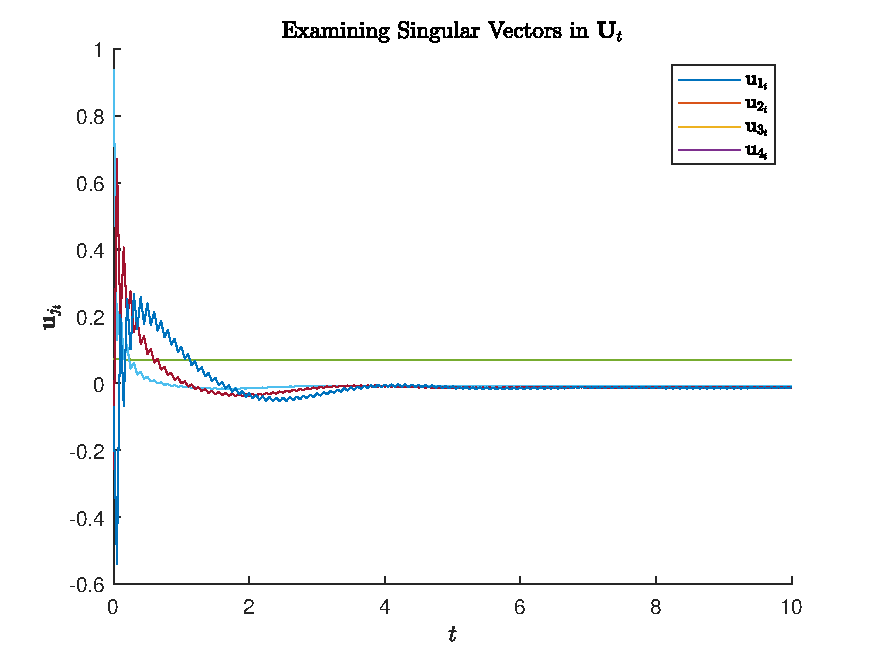
\includegraphics[width=0.48\textwidth]{figures/burgers_ut_1_4.pdf}
        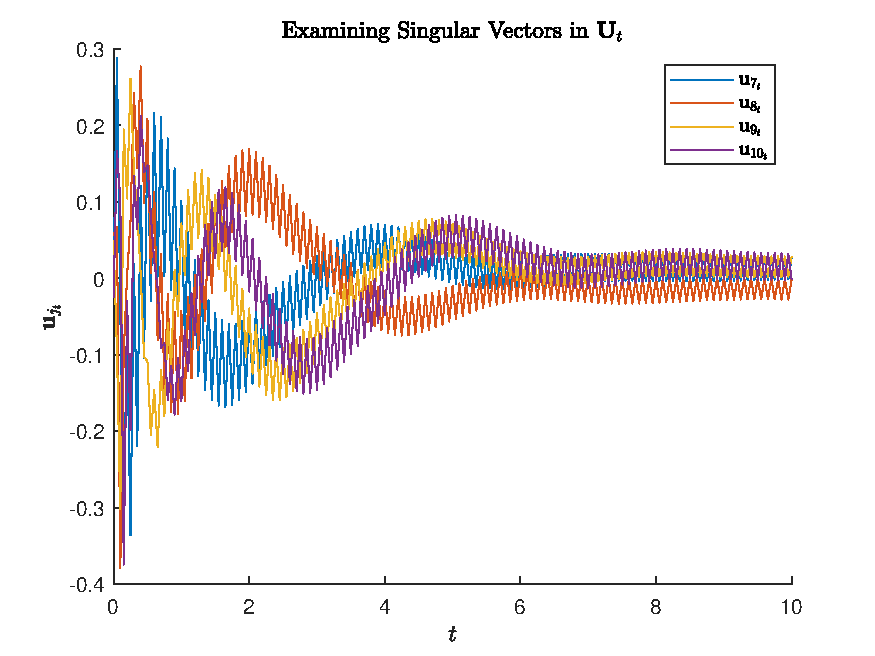
\includegraphics[width=0.48\textwidth]{figures/burgers_ut_7_10.pdf}
        \caption{Examination of $\mathbf{u}_{j_t}$ vectors}
        \label{fig:burgers_ut}
    \end{figure}
    \begin{figure}[t]
        \centering
        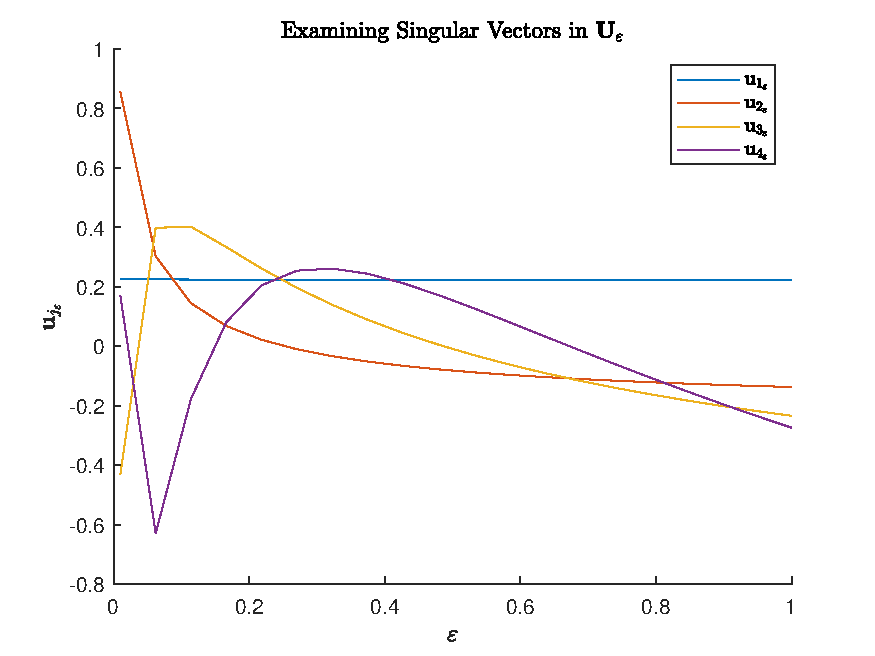
\includegraphics[width=0.48\textwidth]{figures/burgers_ueps_1_4.pdf}
        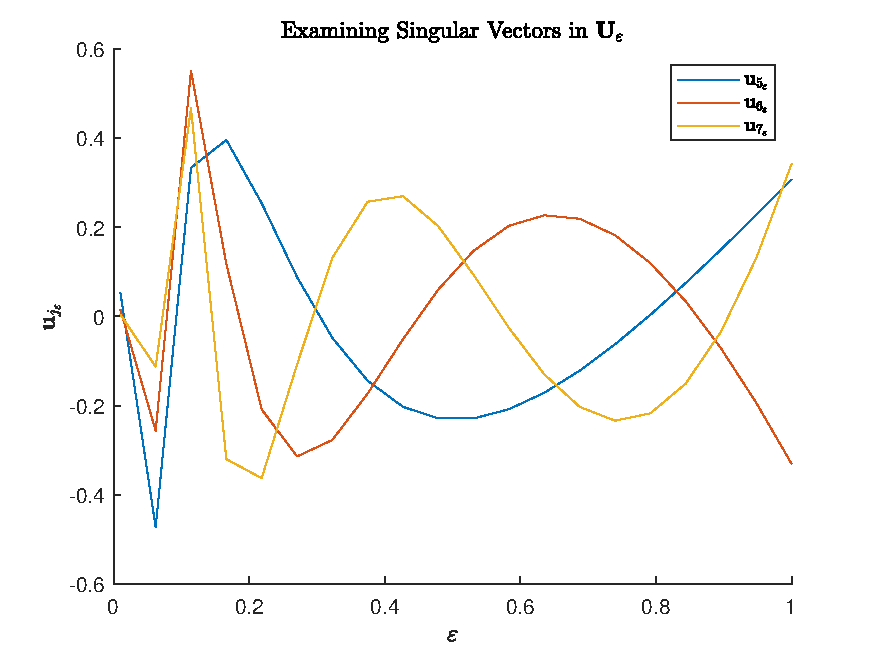
\includegraphics[width=0.48\textwidth]{figures/burgers_ueps_5_7.pdf}
        \caption{Examination of $\mathbf{u}_{j_\eps}$ vectors}
        \label{fig:burgers_ueps}
    \end{figure}

    Analyzing Equation \ref{eqn:burger_def} in $\eps$, we expect extreme sensitivity to perturbation near zero: when $\eps=0$, this becomes a characteristically different PDE, where the time derivative of $w$ is independent of the curvature of $w$ in $x$. Therefore, in Figure \ref{fig:burgers_ueps}, our expectations are met. There are some resolution problems near zero, with possibly chaotic-like behavior, before the vector values smooth out to a polynomial-like function. An improvement, if this simulation were run again, would be to space the epsilon values logarithmically, so the highest concentration of the evaluation points would be near zero and the lowest concentration would be near 1.

    As the only uncompressed variable, $q_1$ seems to provide significant variation not easily captured by the HOSVD of $\Hat{w}$. This prediction of dimensionality is actually complicated by what we see, represented in part by the first six columns in Figure \ref{fig:burgers_uq1}. The first three columns seem to have rigorous polynomial-like structure, with the variation increasing with the number of columns of $\mathbf{U}_{q_1}$. However, in the following columns, the resolution of $q_1$ is a hindrance to the analysis. It generally seems that each column past the second has half a phase more of an oscillation. It's suspected, then, that these could be trigonometric polynomials of increasing degrees. In that scenario, the functions could be easily approximated with $\sin$ and $\cos$ functions. Thus, a thorough examination of fitting ordinary and trigonometric polynomials on data with a higher resolution would be in order.
    \begin{figure}[t]
        \centering
        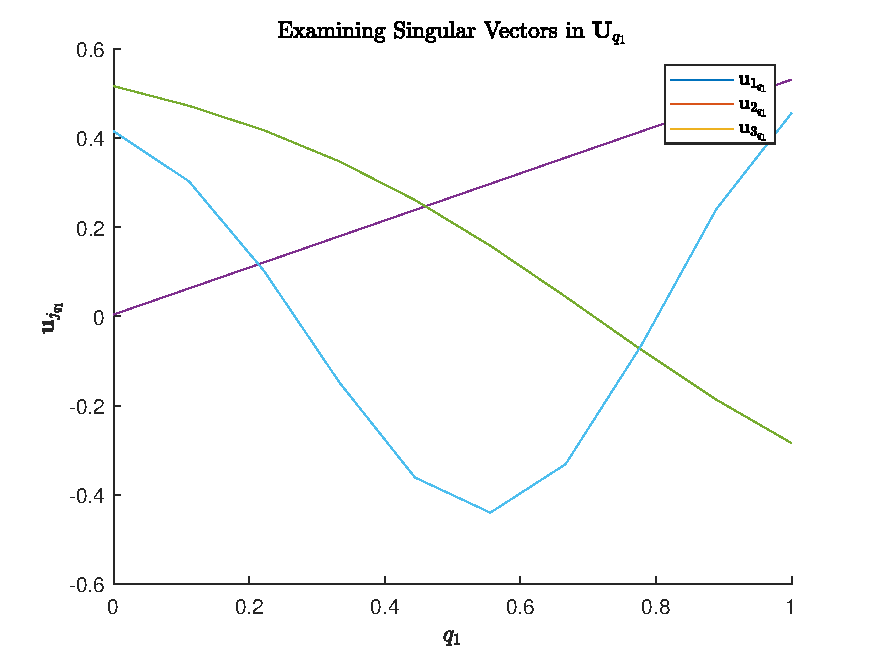
\includegraphics[width=0.48\textwidth]{figures/burgers_uq1_1_3.pdf}
        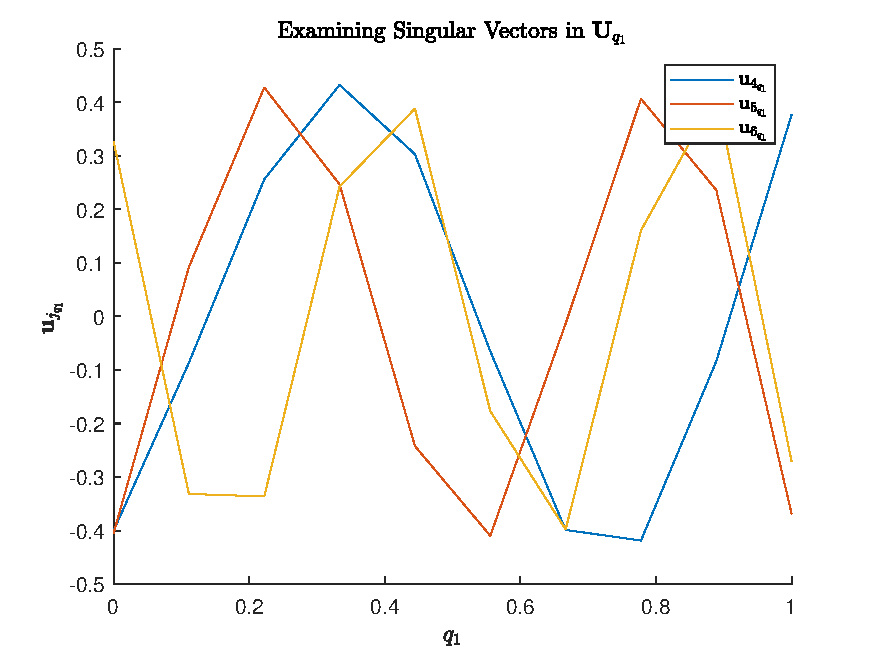
\includegraphics[width=0.48\textwidth]{figures/burgers_uq1_4_6.pdf}
        \caption{Examination of $\mathbf{u}_{j_{q_1}}$ vectors}
        \label{fig:burgers_uq1}
    \end{figure}
    \begin{figure}[t]
        \centering
        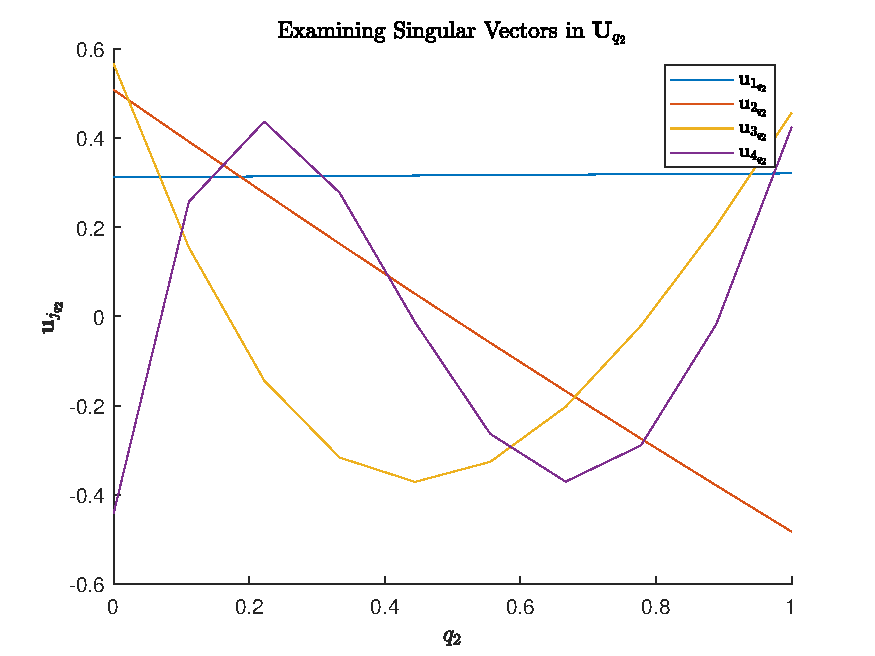
\includegraphics[width=0.48\textwidth]{figures/burgers_uq2_1_4.pdf}
        \caption{Examination of $\mathbf{u}_{j_{q_2}}$ vectors}
        \label{fig:burgers_uq2}
    \end{figure}

    Our last variable, $q_2$, is compressed by $60\%$, and Figure \ref{fig:burgers_uq2} gives a good idea of why it's compressed by such a large proportion. The columns we see here are almost all exactly polynomials of increasing degree or hyperbolic functions, and they are incredibly smooth. The family $\mathcal{F}_{q_2}$ could then feasibly be low-degree polynomials. On a higher level, there seems to be rigorous structure in both $q_1$ and $q_2$, so the initial condition chosen clearly imposes some drastic effects on the solution of the problem. 
    
    \subsubsection{Prediction Performance}
    While the HOSVD works as a method to analyze the structure of Problem \ref{eqn:burger_def}, it doubles as a method for solution approximation. Theoretically, if the solution is simulated for $m_{\eps}\times m_{q_1}\times m_{q_2} = 2000$ different parameter combinations, we'd like to be able to predict a simulated solution in $t,x$ for reasonable choice of $(\Hat{\eps}, \Hat{q}_1,\Hat{q}_2)$. We use two methods of approximation: a linear interpolative method and a method that weights based on proximity to our parameter inputs. Both methods will take inputs of the parameters $\Hat{q}_1,\Hat{q}_2\in(0,1)$, $\Hat{\eps}\in (0.01,1)$ and output a matrix which approximates $w(t,x;\Hat{\eps}, \Hat{q}_1,\Hat{q}_2)$ for $(t,x)\in[0,10]\times[0,1]$. Given $(\Hat{\eps},\Hat{q}_1,\Hat{q}_1)$ and vectors of evaluation points $(\vec{\eps},\vec{q}_1,\vec{q}_2)$, the linear interpolation method will locate the two nearest recorded data points with the smaller's index at $(j_\eps, j_{q_1}, j_{q_2})$, creating a convex combination between them. More specifically, suppose rows $j_\eps,\,j_{q_1},$ and $j_{q_2}$ correspond to the closest evaluated points of $(\eps,q_1,q_2)$. Without loss of generality, suppose $(\Hat{\eps}, \Hat{q}_1,\Hat{q}_2) > (\vec{\eps}(j_\eps),\vec{q}_1(j_{q_1}),\vec{q}_2(j_{q_2}))$ (if not, we change our indexing accordingly). Then, consider the weights
        \[(s_\eps, s_{q_1},s_{q_2}) = \left(\frac{\Hat{\eps}-\vec{\eps}(j_\eps)}{\vec{\eps}(j_\eps+1)-\vec{\eps}(j_\eps)},\;\frac{\Hat{q}_1-\vec{q}_1(j_{q_1})}{\vec{q}_1(j_{q_1}+1)-\vec{q}_1(j_{q_1})},\;\frac{\Hat{q}_2-\vec{q}_2(j_{q_2})}{\vec{q}_2(j_{q_2}+1)-\vec{q}_2(j_{q_2})}\right).\]
    Take $\mathbf{u}^T_{j_\eps}$ as the $j_\eps$th row of $\mathbf{U}_\eps$, then let $\Hat{\mathbf{U}}_\eps = (1-s_\eps)\mathbf{u}^T_{j_\eps} + s_\eps\mathbf{u}^T_{j_\eps+1}$. We create similar $\Hat{\mathbf{U}}_{q_1}$ and $\Hat{\mathbf{U}}_{q_2}$, and then take the tensor
        \[\Hat{\mathscr{T}}_i = \mathscr{C}\times_x \mathbf{U}_x\times_t\mathbf{U}_t\times_\eps\Hat{\mathbf{U}}_\eps\times_{q_1}\Hat{\mathbf{U}}_{q_1}\times_{q_2}\Hat{\mathbf{U}}_{q_2}.\]
    Observe $\Hat{\mathscr{T}}_i\in\R^{n_x\times n_t\times 1\times 1\times 1}$, so the ``interpolation'' approximation $\Hat{\mathscr{T}}_i$ is a matrix approximation of the solution of $w(x,t;\Hat{\eps},\Hat{q}_1,\Hat{q}_2)$.

    The second approximation is equally primitive, but much simpler to explain. A problem with this linear approximation is that it doesn't take into account the ``momentum'' of the solution's change in the parameters $\eps,\,q_1$ and $q_2$; the second method is adjusted to take the solutions for all evaluated values of the parameters into account based on proximity to $(\Hat{\eps},\Hat{q}_1,\Hat{q_2})$. We create column vectors of weights, where the $j_\eps$ weight in $\eps$ will be $\vec{s}_\eps(j_\eps) = |\Hat{\eps}-\vec{\eps}(j_\eps)|^{-1}$, forming $\vec{s}_{q_1}$ and $\vec{s}_{q_2}$ similarly. After normalizing these vectors with respect to the one-norm, the rows of $\mathbf{U}_\eps,\,\mathbf{U}_{q_1},$ and $\mathbf{U}_{q_2}$ are weighted according to the entries in $\vec{s}_\eps,\,\vec{s}_{q_1},$ and $\vec{s}_{q_2}$ (the one norm was chosen in according to how the convex combination in the first approximation ostensibly uses the one-norm, though a different norm choice is a topic to explore). As above, we create $\Hat{\mathbf{U}}_\eps = \vec{s}_\eps^{\;T}\mathbf{U}_\eps$ and make similar $\Hat{\mathbf{U}}_{q_1}$ and $\Hat{\mathbf{U}}_{q_2}$. Then, the tensor
        \[\Hat{\mathscr{T}}_p = \mathscr{C}\times_x \mathbf{U}_x\times_t\mathbf{U}_t\times_\eps\Hat{\mathbf{U}}_\eps\times_{q_1}\Hat{\mathbf{U}}_{q_1}\times_{q_2}\Hat{\mathbf{U}}_{q_2}\]
    will be $n_x\times n_t\times 1\times 1\times 1$, just like $\Hat{\mathscr{T}}_i$. This is denoted the ``proportional'' matrix approximation to $w(x,t;\Hat{\eps},\Hat{q}_1,\Hat{q}_2)$.

    With these approximations, 500 trials were performed to analyze the relative error of the interpolation and proportional approximations from the precise result when plugging in $(\Hat{\eps},\Hat{q}_1,\Hat{q}_2)$ to the simulation. The results of this are shown in Figure \ref{fig:error_hist}, with key numeric data in Table \ref{tab:error_stat}.

    \begin{figure}[h!]
        \centering
        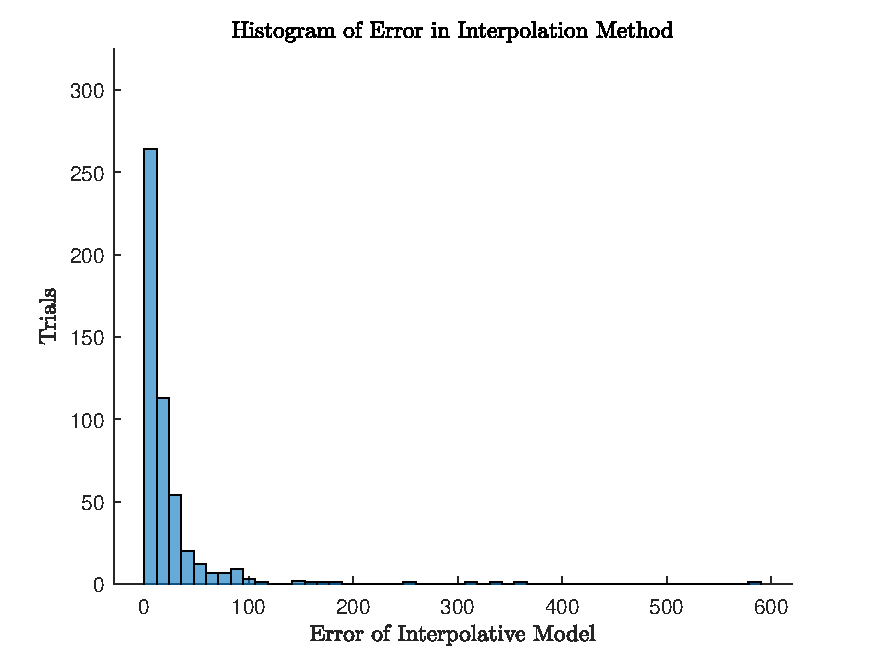
\includegraphics[width=0.48\textwidth]{figures/interp_error.pdf}
        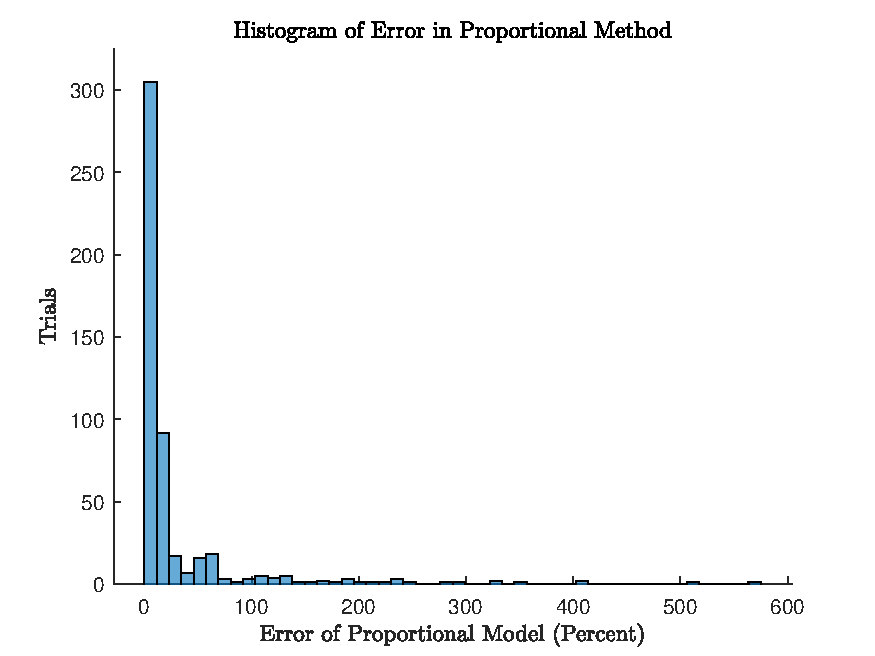
\includegraphics[width=0.48\textwidth]{figures/prop_error.pdf}
        \caption{Error Analysis of Approximations}
        \label{fig:error_hist}
    \end{figure}
    \begin{table}[b]
        \centering
        \begin{tabular}{|| c|c|c|c ||}\hline\hline
            Approximation & Mean Error & Median Error & Standard Deviation of Error\\\hline
            Interpolation & 22.6402$\%$ & 11.3528$\%$ & 43.9937$\%$\\\hline
            Proportional  & 28.8158$\%$ & 8.1058$\%$  & 63.8256$\%$ \\
            \hline\hline
        \end{tabular}
        \caption{Statistics on Approximation Performance}
        \label{tab:error_stat}
    \end{table}

    The upshot is the majority of randomly chosen tuples $(\Hat{\eps},\Hat{q}_1,\Hat{q}_2)$ are approximated fairly well by these methods. However, a clear right-skew is present in both approximation histograms-- there are some factors that clearly cause these outliers affecting the standard deviation to such a great degree. A closer examination of error in each of the variables for any sign of such behavior in Figure \ref{fig:error_vals} gives fine-tuned observations. Just as expected, most parameter triplets result in very low error values, but some important observations stand out. First, there does not seem to be any pattern when examining the error at each choice of $\Hat{\eps}$. Second, the effect of $\Hat{q}_1$ on the error has remarkably well-defined behavior and, as $q_1$ grows, both approximations slowly tend to the simulated solution. Further, the proportional approximation tends to zero much faster, though interpolation minimizes at near interpolation points. Finally, the error explodes for $q_1$ near zero, indicating that more interpolation points near zero would give a better approximation in all likelihood, which is predictable when looking at the information gleaned from Figure \ref{fig:burgers_uq1}. While $q_2$ does not have a clear-cut correlation with the error, it seems that as $q_2$ gets closer to one, the maximal error produced is going to be lower.
    \begin{figure}[h!]
        \centering
        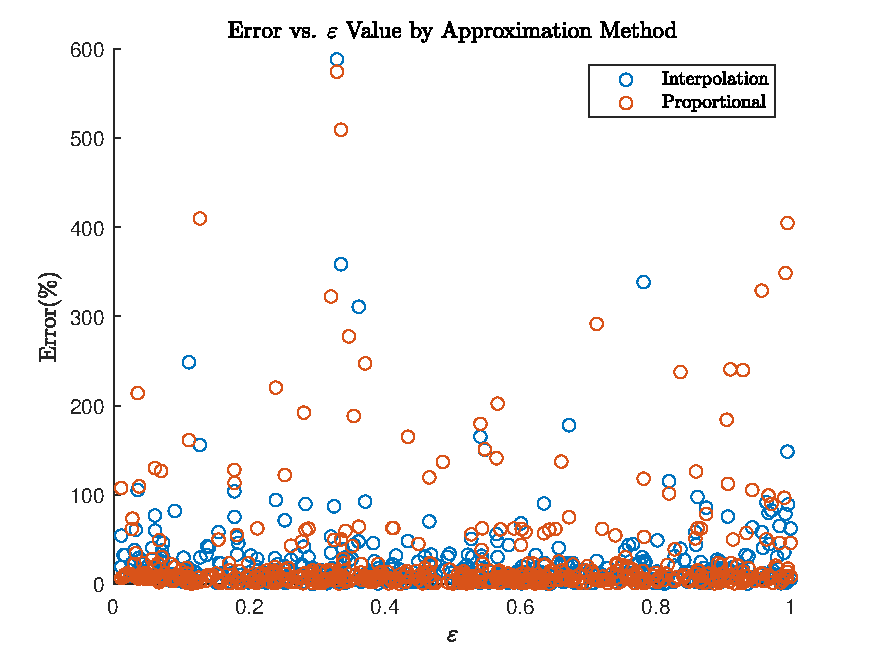
\includegraphics[width=0.48\textwidth]{figures/eps_err.pdf}
        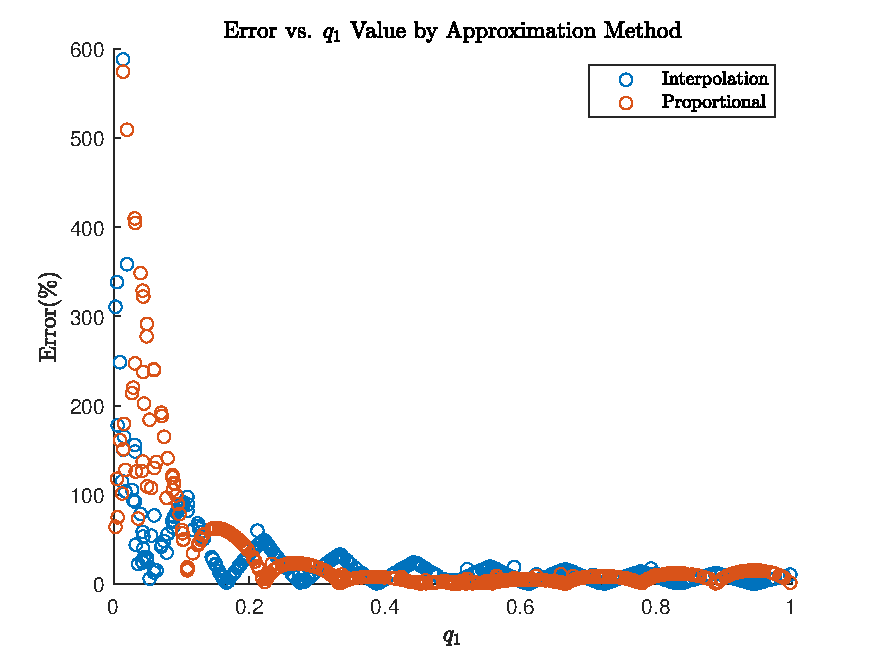
\includegraphics[width=0.48\textwidth]{figures/q1_err.pdf}
        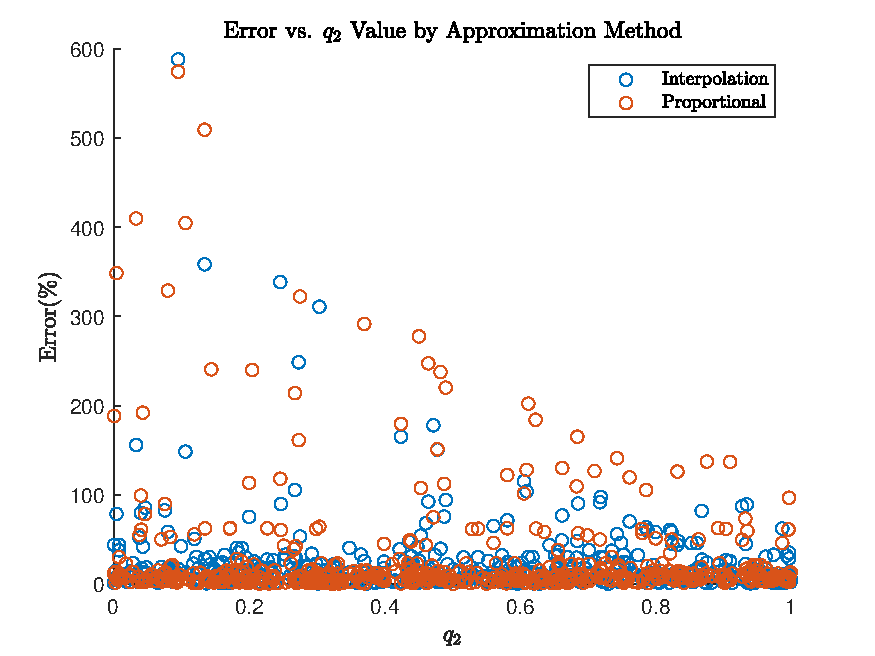
\includegraphics[width=0.48\textwidth]{figures/q2_err.pdf}
        \caption{Error vs Parameter Values}
        \label{fig:error_vals}
    \end{figure}
    
    As a reference, we plot a sample simulated solution $\hat{w}(x,t;\hat{\eps},\hat{q}_1,\hat{q}_2)$ for the arbitrarily chosen unsimulated triplet $(\hat{\eps},\hat{q}_1,\hat{q}_2) = (0.07, 0.42, 0.23)$. An isometric view of the simulation and approximations is displayed in Figure \ref{fig:soln_mesh}. The relative error in the interpolated approximation to the solution is about $15\%$, and the relative error in the proportional approximation to the solution is about $6\%$. This anecdotal and typical example visualizes the error behavior described above, where the proportional approximation is typically closer to the simulated solution than the interpolated solution. Additionally, a large portion of the error seems to be incurred near $t=0$.

    \begin{figure}[t]
        \centering
        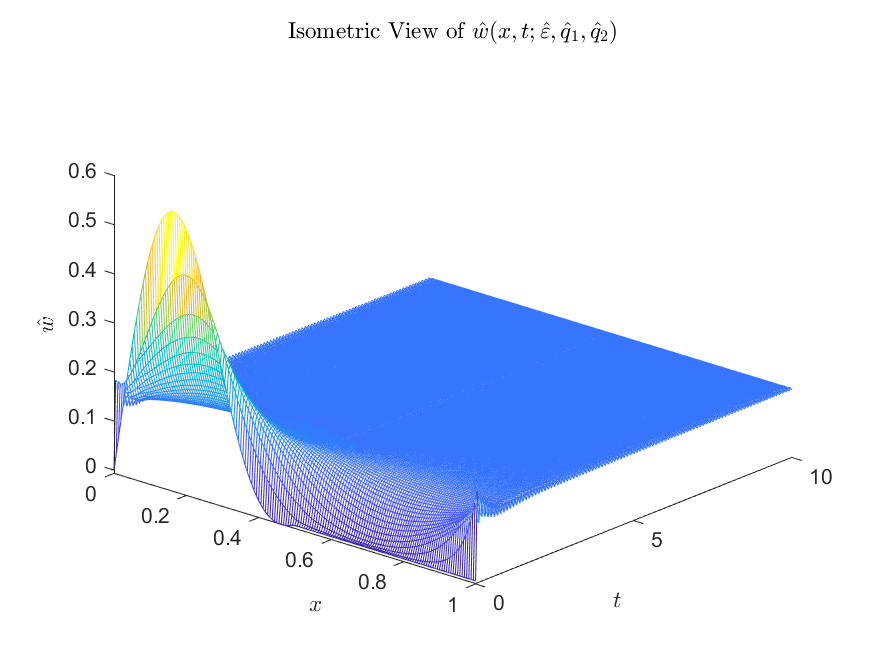
\includegraphics[width=0.48\textwidth]{figures/true_soln.pdf}
        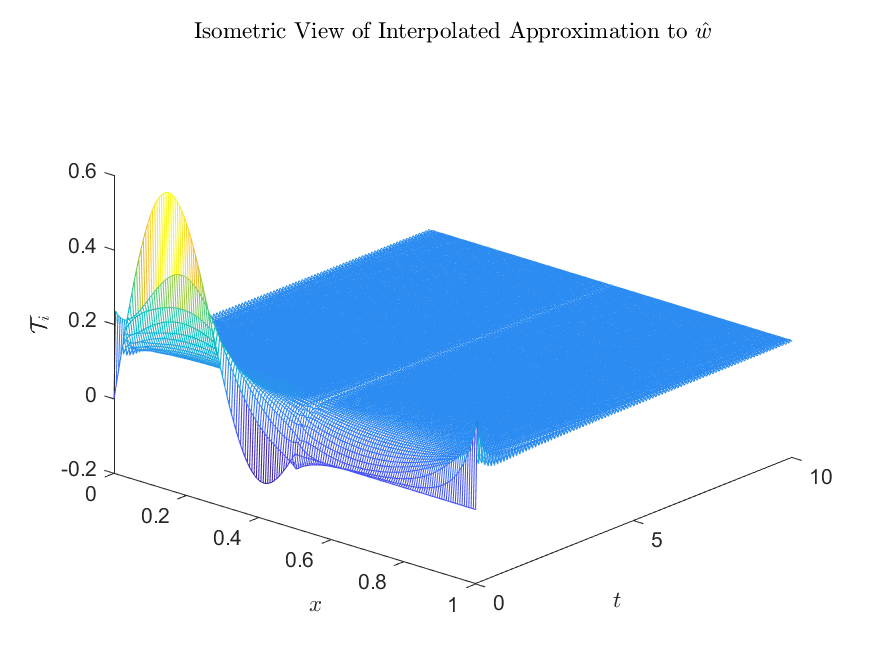
\includegraphics[width=0.48\textwidth]{figures/interp_soln.pdf}
        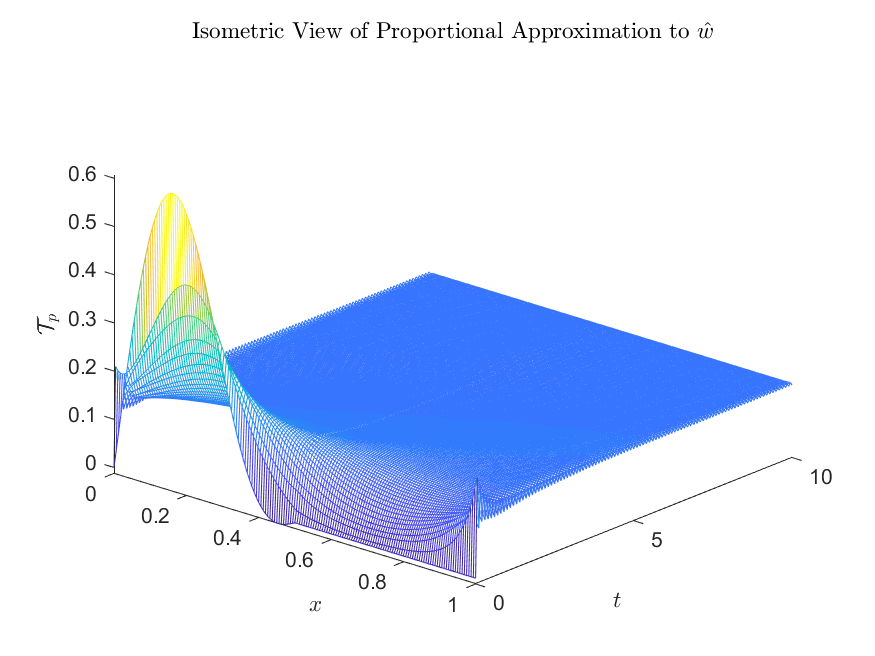
\includegraphics[width=0.48\textwidth]{figures/prop_soln.pdf}
        \caption{Isometric View of Simulated and Approximate Solutions}
        \label{fig:soln_mesh}
    \end{figure}

    \section{Future Work and Conclusion}
    There are several avenues open for further research and numerical experimentation. The first of which is a further structural analysis using the idea of an Analytical HOSVD, which would perhaps give an idea of how to choose $\varphi_{j_k}$ in specific cases, like in Section \ref{sec:structure}, and perhaps choose them analytically. Another venue to pursue is further error analysis in solution prediction and a rigorous comparison with other methods, like POD, and increased resolution of the parameters (specifically $q_1$) in identified problem regions. Attempting different methods of approximation using the HOSVD of the simulations, such as using a hybrid method of the two methods proposed, using different norms, or other more complex methods could decrease the relative error to a solution or its simulation. Finally, fusing the structural analysis portion and the prediction by using a hybrid analytical-numerical HOSVD is a promising path toward accurate prediction. Using spline functions to simulate values of the parameters between the evaluation points and impute data is must less computationally expensive storage- and time-wise to evaluate than any complicated imputation scheme and much more accurate than the current scheme using highly-discretized evaluation points. Overall, there are several promising results from this current exploration, including approximations to piecewise smooth well-defined functions in the structure of the HOSVD and results that line up with expected analytical properties.

    \newpage
    \bibliography{paper} 
    \bibliographystyle{ieeetr}
\end{document}